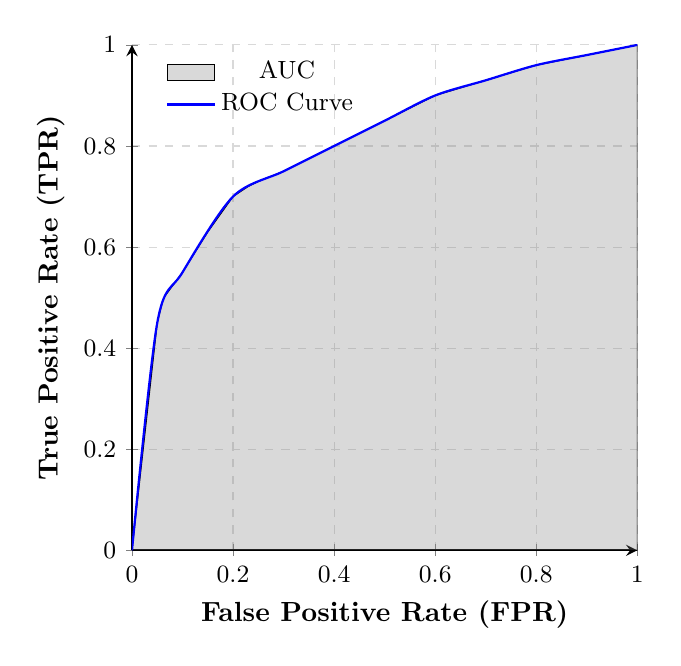
\begin{tikzpicture}
    \begin{axis}[
      width=8cm, height=8cm,
      grid=both, % Adds grid
      grid style={dashed, gray!30},
      xlabel={False Positive Rate (FPR)},
      ylabel={True Positive Rate (TPR)},
      xmin=0, xmax=1, % Limits for x-axis (FPR)
      ymin=0, ymax=1, % Limits for y-axis (TPR)
      axis lines=left,
      axis line style={thick},
      label style={font=\bfseries},
      tick label style={font=\small},
      xtick={0,0.2,0.4,0.6,0.8,1}, % X-axis ticks
      ytick={0,0.2,0.4,0.6,0.8,1}, % Y-axis ticks
      legend style={at={(0.05,0.99)},anchor=north west,draw=none,fill=none, font=\small}
    ]
  
    % Shaded area under the ROC curve (AUC) with improved precision
    \addplot[
      domain=0:1,
      samples=200,
      fill=gray,
      fill opacity=0.3,
      area legend
    ]
    coordinates {
      (0,0) (0.05,0.45) (0.055,0.47) (0.06,0.49) (0.063,0.5) (0.1,0.55) (0.15,0.63) (0.2,0.7) (0.23,0.72) (0.25,0.73) (0.3,0.75) (0.4,0.8) (0.5,0.85) (0.6,0.9) (0.7,0.93) (0.8,0.96) (0.9,0.98) (1,1) (1,0) (0,0)
    };
    \addlegendentry{AUC}
  
    % Plotting the ROC curve for a typical classifier with a thicker line
    \addplot[thick, smooth, blue] coordinates {
      (0,0) (0.05,0.45) (0.1,0.55) (0.2,0.7) (0.3,0.75) (0.4,0.8) (0.5,0.85) (0.6,0.9) (0.7,0.93) (0.8,0.96) (0.9,0.98) (1,1)
    };
    \addlegendentry{ROC Curve}
  
    \end{axis}
  \end{tikzpicture}